\section{Experiments}
\label{sec:experiments}

%\mb{I find ``\emph{around-right}'' more informative as a name than
%  ``\emph{template}''. I am replacing it in the text, but it should
%  also be updated in the figures.}

% We conducted three different experiments where we evaluated the accuracy of the models in terms of how many test commands were exactly translated
% into corresponding test actions. 
% \citet{Lake:Baroni:2017} found that RNNs models are achieve nearly perfect performance when tested on a random split of SCAN but accuracy drops significantly
% (down to around 20\% for their best performing model) when the network is tested on composing new meanings after being exposed only to shorter samples.

% In order to make our results comparable with previous work on SCAN each training set consists of 100,000 examples sampled with replacement
% from each related train/test split. We decided to replicate experiment 1 of \cite{Lake:Baroni:2017} that simply uses a random split
% of the SCAN dataset divided into a train (80\%) and test (20\%) set. This would act as a first comparison with the RNNs results reported in their work.

% \subsection{Experiment 1: random split and primitive generalization}
% \label{subsec:exp1}

\subsection{General results}

%\mb{Please add table with our results for the 3 splits for both the
%  best-overall and the split-best settings (and sds), as well as the
%  L\&B, Loula et al and Bastings et al results (for the latter, the
%  GRU+att 12.5 jump result should suffice.}

\begin{table*}[t!]
    \footnotesize
    \centering
        \begin{tabular}{l |l| l | l}
             & \textbf{Random} & \textbf{Jump} & \textbf{Around Right} \\ \hline
             LSTMs \cite{Lake:Baroni:2017} & 99.8\% & 1.2\% & -- \\
             LSTMs \cite{Loula:etal:2018} & -- & -- &  2.46\% $\pm$ 2.68\% \\
             GRUs \cite{Bastings:etal:2018} & \textbf{100.0\%} $\pm$ 0.0\% & 12.5\% $\pm$ 6.6\% & --  \\
             \hline
             CNNs & 99.97\% $\pm$ 0.03\% & \textbf{69.24\%} $\pm$ 8.17\%  & \textbf{56.7\%} $\pm$ 10.24\% \\
        \end{tabular}
    \caption{\label{table:main results} \rd{I will fix both tables so that at least one of them fit on one column.} Test performance for the three splits used in our experiment 1. For \newcite{Lake:Baroni:2017} 
    we report results from their best model on every split
    which had higher performance then their best overall model.}
\end{table*}



Table \ref{table:main results} summarizes our main results. Like the RNNs studied by
\newcite{Lake:Baroni:2017}, our CNN has no problem in the
\emph{random} split. However, its results are also much higher than
those of the best RNNs for the compositionally challenging \emph{jump}
and \emph{around-right} splits. This suggests that, in principle, CNNs
hold more promise as deep networks able to acquire systematic
generalization. Still, in neither challenge we observe the perfect
performance we should expect if networks had extracted and where
applying the correct symbolic rule. Indeed, qualitative analysis of
the errors do not suggest rule-based learning. It is not the case, for
example, \mb{add some qualitative error analysis.}

Moreover, as Fig.~\ref{fig:exp1} shows, there is a big difference in
stability between \emph{random} and the other splits. This figure
reports mean cross-seed accuracy and the corresponding standard
deviation for the top 10 configurations for each split. The
\emph{random} results are very stable across seeds and
hyperparameters. \emph{Jump} accuracy is relatively stable across
hyperparameters, but has large variance across seeds. For the most
challenging \emph{around-right} split, we observe instability both
across seeds and hyperparameters (although even the lowest end of the
reported accuracies is always well below the best RNN performance in
the corresponding experiments).

Another question is whether the best configurations are coherent
across splits, or each split requires an ad-hoc hyperparameter setting
that does not generalize to the other tests. We find that overall this
is not the case, and it is possible to find configurations that
achieve good performance across the 3 splits. In particular, the
\emph{best overall configuration}, that we take as the starting point
for further experiments below, has a learning rate of 0.01, 25 tokens
batch size, 0.25 dropout, 6 layers in both the encoder and the
decoder, 512 embedding dimensionality, and convolutional kernel width
5. Such model was ranked 13th best (of about 2.5K explored) on the
\emph{random} split (with a mean cross-seed accuracy of 99.92\% off by
0.05\% from the top configuration for the split), 32th on the
\emph{jump} split (60.67\% mean accuracy, off by 8.62\%), and 2nd in
the \emph{around-right} split (mean 53.25\% accuracy, off by
3.45\%). 
\rd{from here} We found the best overall model by first selecting only the models
that ranked 300th or higher in all three splits. Then for every model
we selected the lowest rank (low-rank) among the three split and we picked 
as best overall the model with the highest low-rank. As an example, if only
two models were among the top 300 on all three splits and model \textit{A} was
ranked 1st, 2nd and 50th on random, jump and around-right respectively, and model \textit{B}
ranked 45th, 10th and 10th then model \textit{A} would have a low-rank value of 50 and
model \textit{B} a low-rank value of 45. Model B would then be selected as best overall model.

\mb{Should we say how the best overall was found?} \rd{to here. Does it make sense?}
% Experiment 2 and 3 in section \ref{subsec:exp2} and \ref{subsec:exp3} used the aforementioned model.

% After a preliminary experiment we found a subset of parameters showing reasonable performance and conduceted a large hyperparameters
% search on every split.
% We varied batch sizes (in term of number of tokens in the batch: 25, 50, 100, 200, 500 and 100), learning rates
% 0.1, 0.01, 0.001), the embedding dimensions (128, 256, 512), amount of dropout used (0, 0.25, 0.5) \cite{srivastava:eta:2014}, number of convolutional
% layers for both the encoder and decoder (6, 7, 8, 9, 10) and width of the convolutional kernel (3, 4, 5).
% We then cross validated the top-300 models across 5 different runs. Accuracy and standard deviation are presented in figure \ref{fig:exp1}. 
% We inspected the average accuracy of the model note that the amount of standard deviation of the top-300 models reached a performance range with a lower limit that was always
% considerably lower than the best model for each split, making us think that considering the top-300 models was
% a right choice that included tha real best model for every split. In other words, the accuracy for the best model and the 300th one formed a large range.
% \footnote{This might not seem the case for the results on the random split where the range is (95.17, 99.97). However the standard deviation across all 300 models does not
% exceed 2.7}
% When analyzing the the resulting models for every split we computed a \textbf{best overall model} across all splits which
% was a model trained with a learning rate of 0.01, a 25 tokens per batch, dropout applied with probability 0.25, it had 6 layers in both the encoder and the decoder,
% embedding dimension of 512, a convolutional kernel of width 5. Such model was ranked 13th on the random split (with an accuracy of 99.92\% off by 0.05\%), 
% 32th on the jump split (60.67\% accuracy, off by 8.62\% compared to the top performing model for the split),
% and 2nd in the template split (53.25\% accuracy, off by 3.45\%)
% Experiment 2 and 3 in section \ref{subsec:exp2} and \ref{subsec:exp3} used the aforementioned model.

\begin{figure}[tb]
    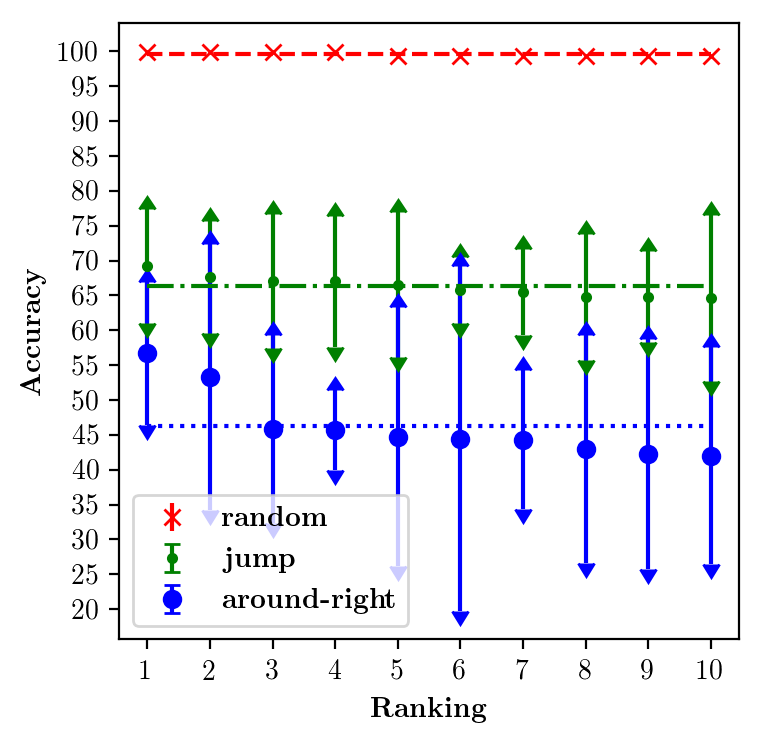
\includegraphics[width=.5\textwidth,keepaspectratio]{figures/accuracies_all_splits.png}
    \centering
    \caption{Accuracies (\%) of top-10 models on random, jump and around-right (arrows
      denote standard deviations). Dashed lines report average accuracy
      of the models on every split.
      % \mb{means across what? Also, it would be better if
      %legend order was random/jump/around-right}
      }
    \label{fig:exp1}
\end{figure}

\begin{figure}[h]
    \centering
    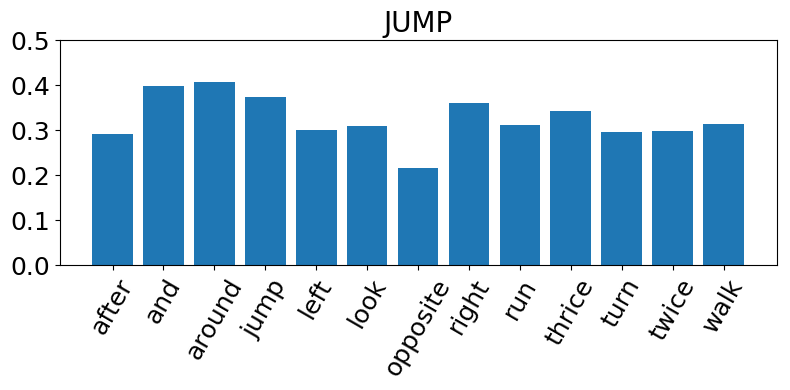
\includegraphics[width=.4\textwidth,keepaspectratio]{figures/jump_error_dist.png}
    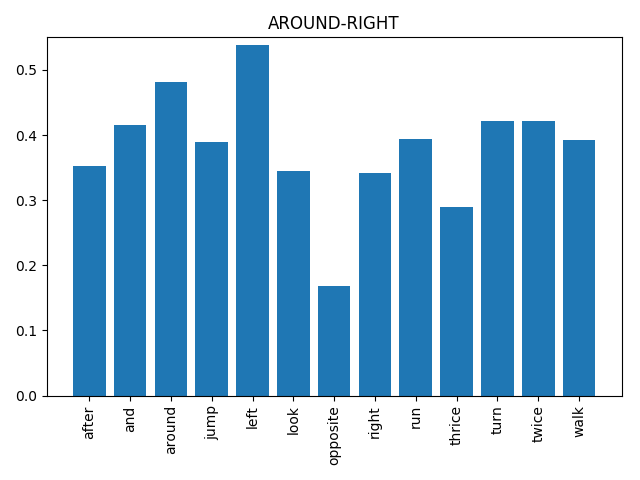
\includegraphics[width=.4\textwidth,keepaspectratio]{figures/template_error_dist.png}
    \caption{Proportion of commands with a certain word (over word
      total) that were wrongly executed by the respective best CNNs in
      the \emph{jump} (t) and \emph{template} (b) splits.}
    \label{fig:error_distributions}
\end{figure}


Although the CNNs dramatically outperform the RNNs, their performance
is still far from perfect (cf.~\label{table:main results}). The SCAN
tasks are designed to be easy for a system that has learned the right
composition rules. Perhaps, CNN's performance is not perfect because
they only learned a subset of the necessary rules. For example, they
might be able to correctly interpret the new expression \emph{jump
  twice} because they induced a \emph{X twice} rule from their
training set, but they might fail at \emph{jump thrice} because they
failed to learn the corresponding \emph{X thrice} rule. Since SCAN
semantic composition rules are associated with single words in input
commands, we can check this hypothesis by looking at error
distribution across input words. It turns out that, in neither the
\emph{jump} nor the \emph{around-split}, errors are strongly
associated to specific input commands. Figure
\ref{fig:error_distributions} shows proportion of errors in commands
containing a word (over total occurrences of the word) made by the
best models in each split. Besides observing that \emph{opposite} is
consistently easier, we observe a relatively stable proportion of
errors across command words (the hardest word, \emph{left} in the
\emph{around-right} split, is wrongly executed in 54\% of the cases in
which it occurs). Direct inspection of the errors reveals no traces of
systematicity. Indeed, we often find minimal pairs in which changing
one action verb with another (distributionally equivalent in SCAN)
turns a correctly executed command into one where the CNN fails. For
example, in the \emph{jump} split, the CNN correctly executes
``\emph{jump left after walk},'' but fails ``\emph{jump
  left after run}'' (jumping is forgotten). Analogously, in the
\emph{around-right} split, ``\emph{run around right}'' is correctly
executed, but ``\emph{walk around right}'' isn't (the CNN stops too
soon).


\subsection{Impact of kernel width}
\label{subsec:exp2}

One important difference between recurrent and a convolutional
architectures is that the former read an item at the time, and it is
left to the learned dynamics of the recurrent matrix to determine
context width, whereas the kernel width of a CNN imposes a strong
prior on the window of elements to be processed together. We
conjecture that relatively wide encoder and decoder widths, by
naturally pushing the network to keep wider contexts into account,
might favour the acquisition of template-based generalizations, and
hence better compositionality. To investigate this hypothesis
empirically, we tested the best-overall model varying both encoder and
decoder widths between 1 and 5.\footnote{At least on the encoder side,
  larger widths seem excessive, as the longest commands are
  9-word-long.}

% We consider the use of convolutional filters as an interesting dimension to inspect, especially when considering 
% its ability to possibly assess the small and self contained semantics of single words within the larger context of a sentence \rd{\dots make a proper example with SCAN]}.
% The desired systematic compositionality that we seek to find in modern neural networks could indeed be described as the
% human ability to extract, process and combine small unit that are semantically meaningful, in order to create a larger and again meaningful semantic block.
% The hypothesis of the use of convolutions as an important parameter for the ability of the network
% to correctly process semantic compositionality is investigated in our second experiment presented in section \ref{subsec:exp2}.

\begin{figure*}[tb]
    \centering
    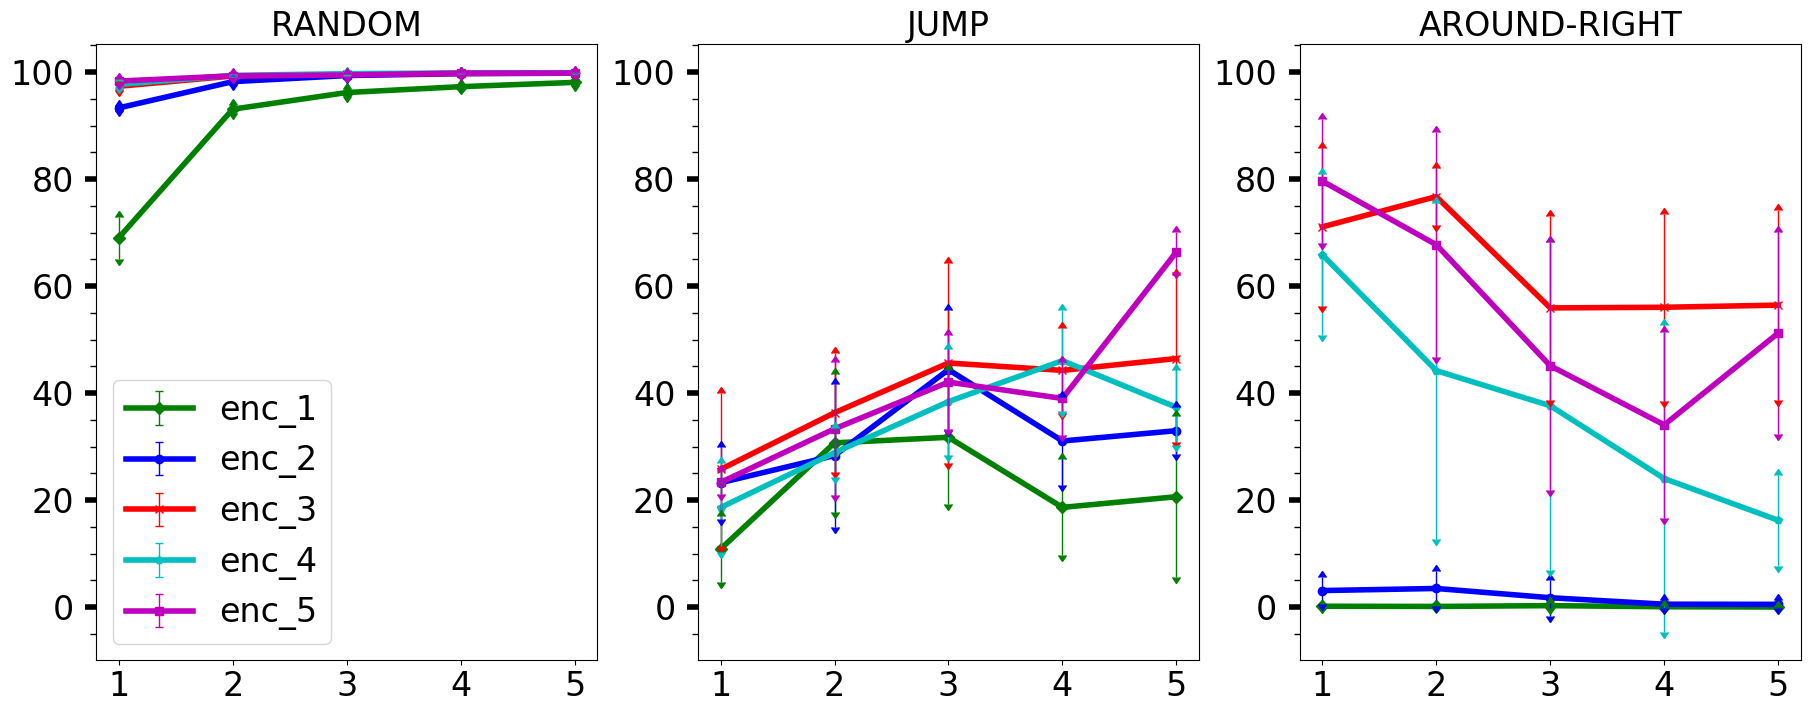
\includegraphics[width=\textwidth,keepaspectratio]{figures/kernel_exp.png}
    \caption{Mean accuracies (\%) across 5 seeds for each split, in function of decoder (x axis) and encoder (colors) kernel widths. Arrows denote standard deviations.
    %More natural order would be random/jump/around-right.
    \mb{Also crop actual file and enlarge figure.}
    }
    \label{fig:kernel_exp}
\end{figure*}

In the \emph{random} split, as expected, both wider encoder and
decoder windows lead to better performance. The \emph{jump} results
follow the same train, although in a less clear-cut way. Still, the
narrowest encoder-decoder combination shows the worst performance, and
the widest kernel combination the top one. For the
\emph{around-right} split, it's also better to use the widest encoder,
but top performance is achieved with the \emph{narrowest} decoder
(width$=$1). Indeed, with the narrow decoder we obtain
\emph{around-right} accuracies that are even above the absolute-best
\emph{jump}-split performance. Since the novel output templates in the
\emph{around-right} split are by construction long (they involve
executing an ``around'' command that involves repeating an action 4
times), we would have rather expected models keeping track of a larger
decoding window to fare better particularly in this case.

To gain some insight on the attested behaviour, we looked at
performance in function of ground-truth output length in the two
splits. Keeping encoder width fixed at 5, Fig.~\ref{fig:kernel_width}
reports the proportions of cases that were correctly handled only with
decoder width 1, 5, both or neither, considering models trained on
\emph{jump} and \emph{around-right}. We plot statistics for the cases
at intersection of the two split test sets, but the same pattern is
confirmed when looking outside this intersection. We observe more
cases where both widths work in the \emph{around-right} split, showing
that overall it is less damaging to use the wider kernel with
\emph{around-right} than the narrower one with \emph{jump} (see also
Fig.~\ref{fig:kernel_exp}). In general, though, we find that the
wide-decoder \emph{jump} model behaves quite similarly to the
narrow-decoder \emph{around-right} model, getting most of its gains
from shorter sequences. One interesting difference is that, for
\emph{around-right}, we observe an inversion in performance for the
longer sequences, where the wider decoder outperforms the narrower
one, in accordance with our intuition that more context should help
longer execution tasks. Looking qualitatively at the errors, we note
that, for both splits, the narrower decoder tends to skip trajectory
sub-chunks (e.g., executing ``jump around right'' with 3 instead of 4
right turns followed by jumps), whereas the wider kernel is more
likely to substitute actions (e.g., turning left instead of right)
than undershooting the length. This impressionistic observation is
supported by the fact that, for both splits, the narrow-kernel errors
have considerably larger variance with respect to ground-truth
length. While these analyses confirm the fact that a wider decoder
kernel helps with length management, we still have no insight on why
the shorter kernel should be better on the around-right split. Future
work should pursue a better understanding of how kernel widths affect
linguistic processing in CNNs.

\begin{figure}[tb]
    \centering
%    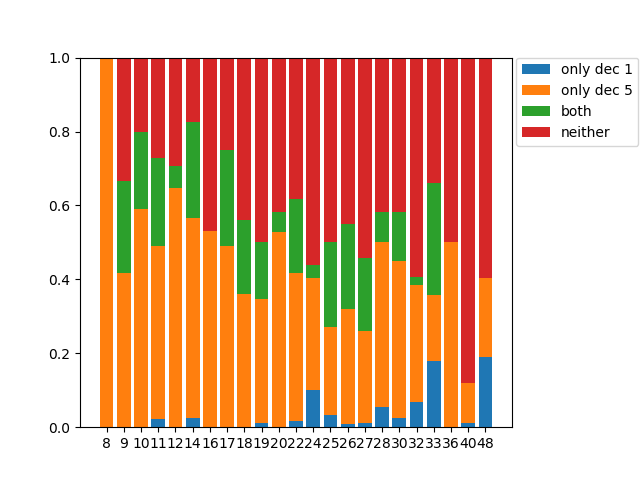
\includegraphics[width=.4\textwidth,keepaspectratio]{figures/jump_subset_out.png}
%    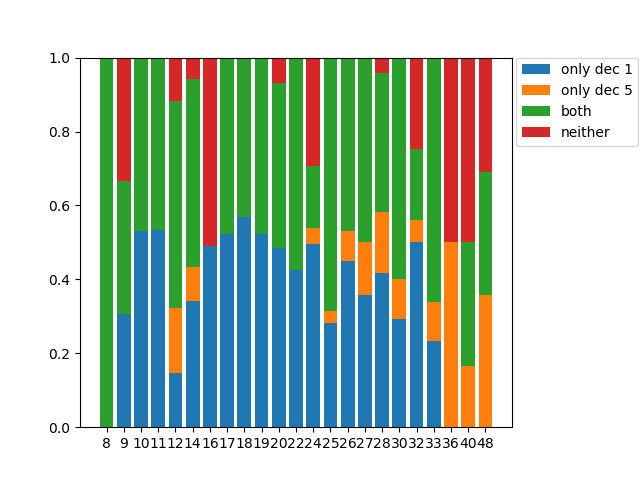
\includegraphics[width=.4\textwidth,keepaspectratio]{figures/template_subset_out.png}
    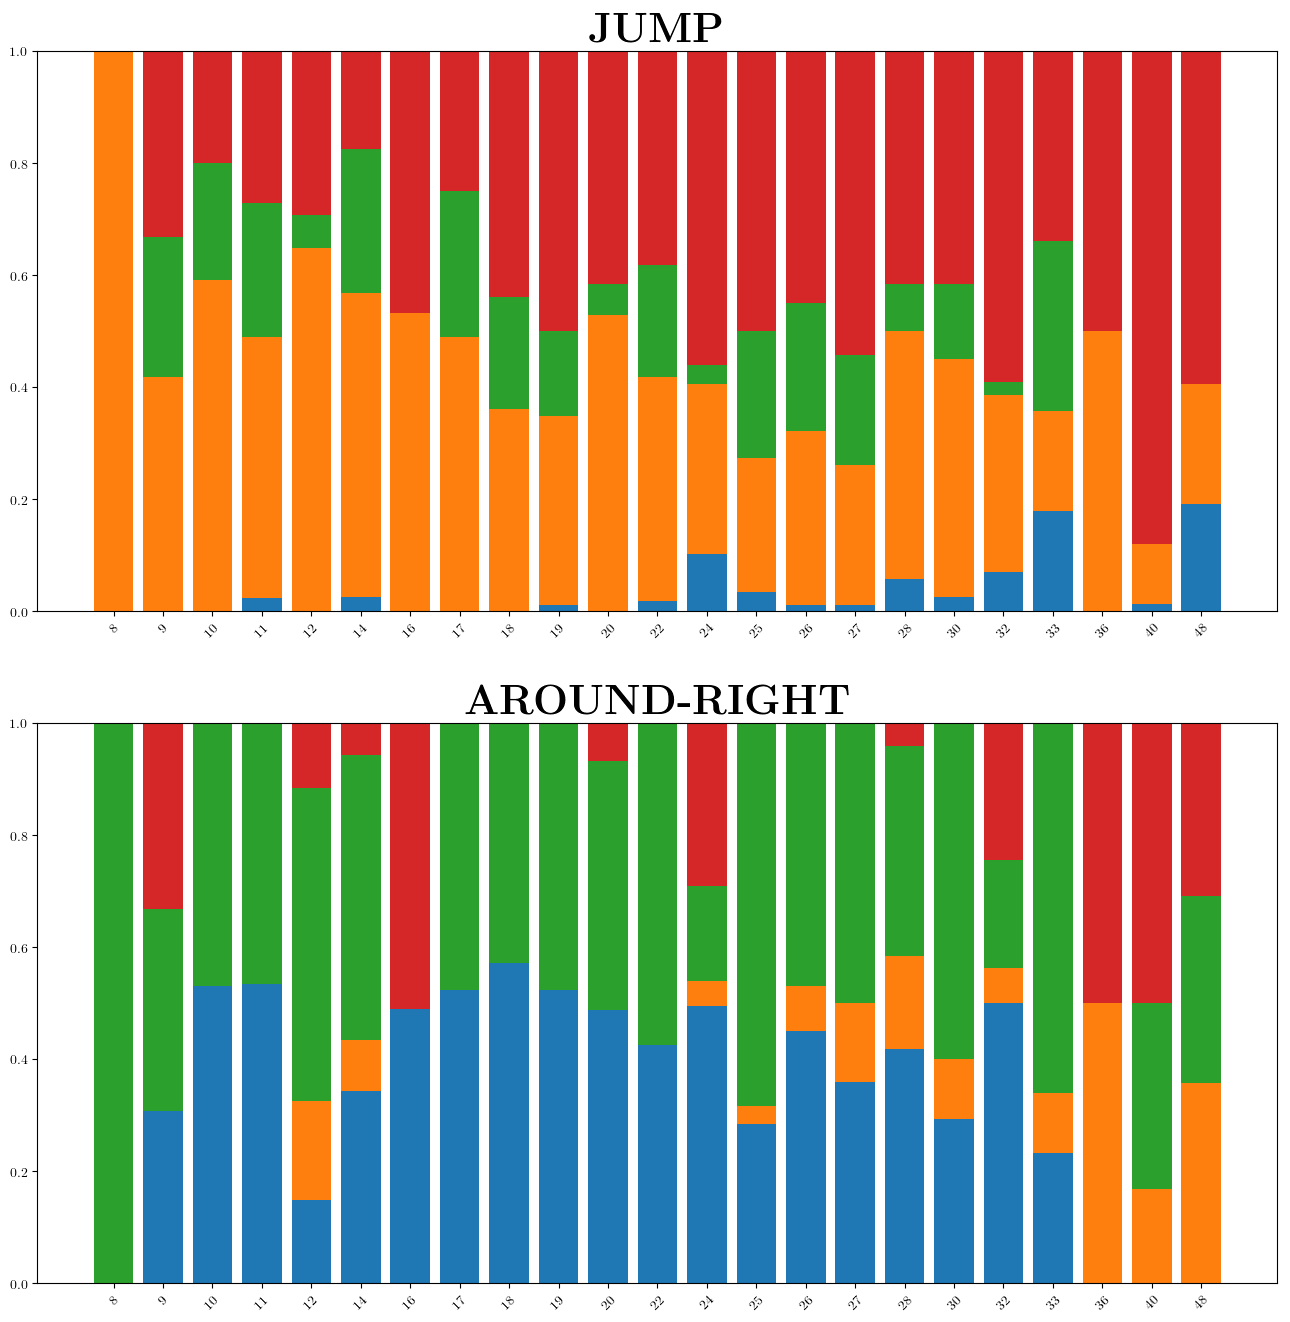
\includegraphics[width=.5\textwidth,keepaspectratio]{figures/split_subset_out.png}
    \caption{Proportion of items that were correctly executed by
      models with 5- and 1-decoder widths, in function of ground-truth
      output length.}
    \label{fig:kernel_width}
\end{figure}

\subsection{Impact of multi-layer attention}
\label{subsec:exp3}

Finally, as attention is the only component linking encoder and
decoder in CNNs and other non-recurrent architectures, we looked more
in-depth at whether the multi-layer attention mechanism of the fairseq 
CNN implementation we are using is important, or attention from a
single/fewer decoder layers could suffice. Results are presented in
\ref{fig:exp3}.

\begin{figure}[tb]
    \centering
    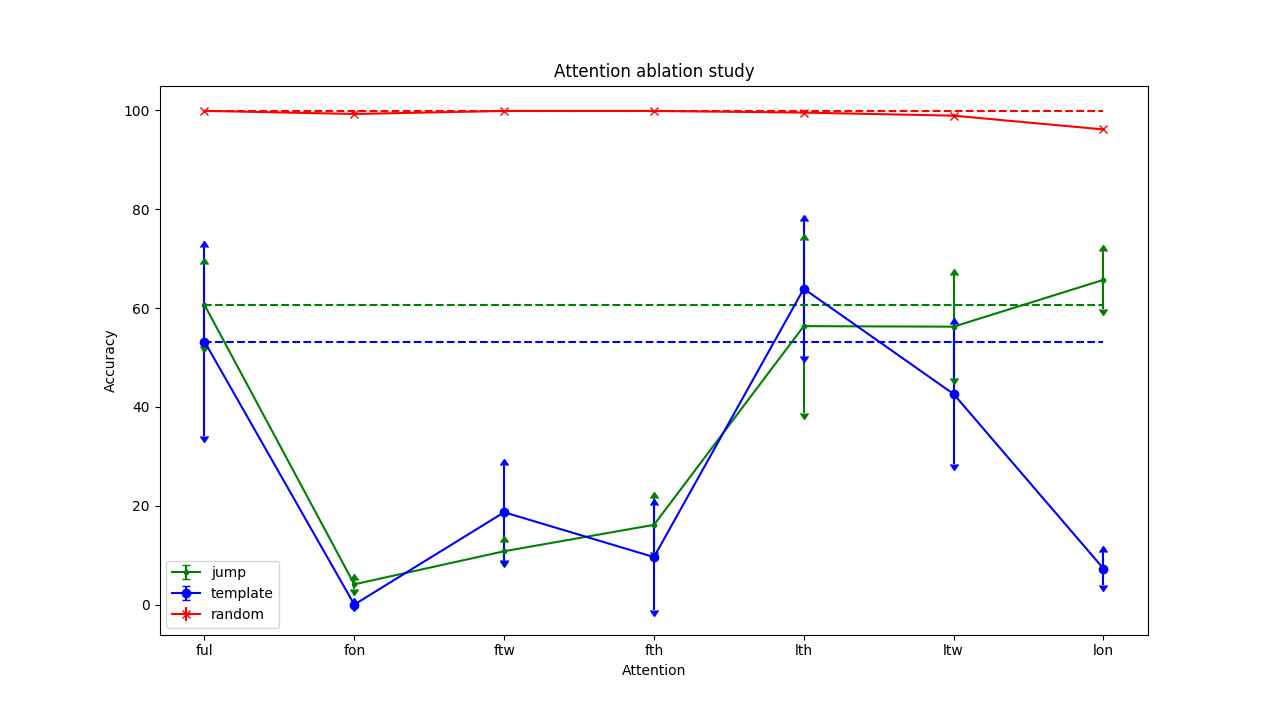
\includegraphics[width=.5\textwidth,keepaspectratio]{figures/attention_exp.png}
    \caption{Accuracy for attention experiment. Dashed lines reports accuracy with attention on every layer}
    \label{fig:exp3}
\end{figure}

